%\documentclass[11pt, twocolumn]{article}
\documentclass[11pt,a4paper]{article}
%\usepackage[top=0.85in,left=2.75in,footskip=0.75in]{geometry}
\usepackage[top=1in,bottom=1in]{geometry}

% Use adjustwidth environment to exceed column width (see example table in text)
\usepackage{changepage}

% Use Unicode characters when possible
\usepackage[utf8x]{inputenc}

% textcomp package and marvosym package for additional characters
\usepackage{textcomp,marvosym}

% cite package, to clean up citations in the main text. Do not remove.
%\usepackage{cite}

% line numbers
\usepackage[right]{lineno}

% ligatures disabled
\usepackage{microtype}
\DisableLigatures[f]{encoding = *, family = * }

% color can be used to apply background shading to table cells only
\usepackage[table]{xcolor}

% array package and thick rules for tables
\usepackage{array}

% create "+" rule type for thick vertical lines
\newcolumntype{+}{!{\vrule width 2pt}}

% Bold the 'Figure #' in the caption and separate it from the title/caption with a period
% Captions will be left justified
%\usepackage[aboveskip=1pt,labelfont=bf,labelsep=period,justification=raggedright,singlelinecheck=off]{caption}
\usepackage[aboveskip=1pt,labelfont=bf,labelsep=period,singlelinecheck=off]{caption}
\renewcommand{\figurename}{Fig}

% Bibliography related
\usepackage[round,numbers,sort&compress]{natbib} 
\bibliographystyle{unsrtnat}

% Graphics
\usepackage{graphicx,color}% Include figure files
\usepackage{epstopdf}

% Misc.
%\usepackage{adjustbox}

% Math
\usepackage[intlimits]{amsmath}
\usepackage{amsfonts}
\usepackage{bm}
\usepackage{amssymb}
\usepackage{mathtools}


% Title, Authors, etc.
\title{BioExcel use case for PMF calculations with GROMACS}
\usepackage{authblk}

% Leave date blank
%\date{}
\author{Viveca Lindahl}

\begin{document}
\maketitle
\tableofcontents

\section{Background}
Calculating free energy (FE) differences between different conformational states is central to molecular dynamics (MD) simulation studies of biological systems. The GROMACS simulation software package is capable of carrying out efficient and highly parallel computations. However, for a large-scale study there are many technical steps on the way posing significant barriers for the non-expert user. Figure~\ref{fig:mdworkflow} shows a typical MD workflow -- using experimental data combined with modeling as input, the goal is to  make novel predictions or observations inaccessible to real-life experiments. The simulation component of the workflow has significant complexity that is currently not automated and requires time-consuming planning and management from the user. The scientific question typically involves comparing different molecular systems, e.g. different compounds in drug discovery, different sequences and mutations in DNA and protein studies, multiplying the number of simulations (by a number $n_0$, in Fig~\ref{fig:mdworkflow} -- TODO). In addition, one would apply  different simulation conditions, e.g. varying the force field model to gauge the universality of the results ($n_1$). Furthermore, the full simulation setup should be replicated in order to obtain reliable estimates of the statistical uncertainty, further multiplying the number of simulations ($n_2$).  Also, in particular for FE calculations, efficient sampling is key. For finite simulation times complex system get trapped in metastable states, yielding unreliable statitsics. However, sampling can be enhanced by advanced sampling techniques that typically exploit non-equilibrium sampling in combination with bias potentials to promote transitions between metastable states. The efficiency of such methods can further be improved by simultaneously launching multiple ($n_3$) communicating trajectories, also known as ``walkers'', that share the sampled data on-the-fly, enabling more efficient extraction of information. Because of the complexity of this workflow, it is non-trivial to both design and carry out MD simulations. 

\begin{figure*}[thbp!]
%\includegraphics[width=1\textwidth]{figs/config.pdf}                                                                                                           
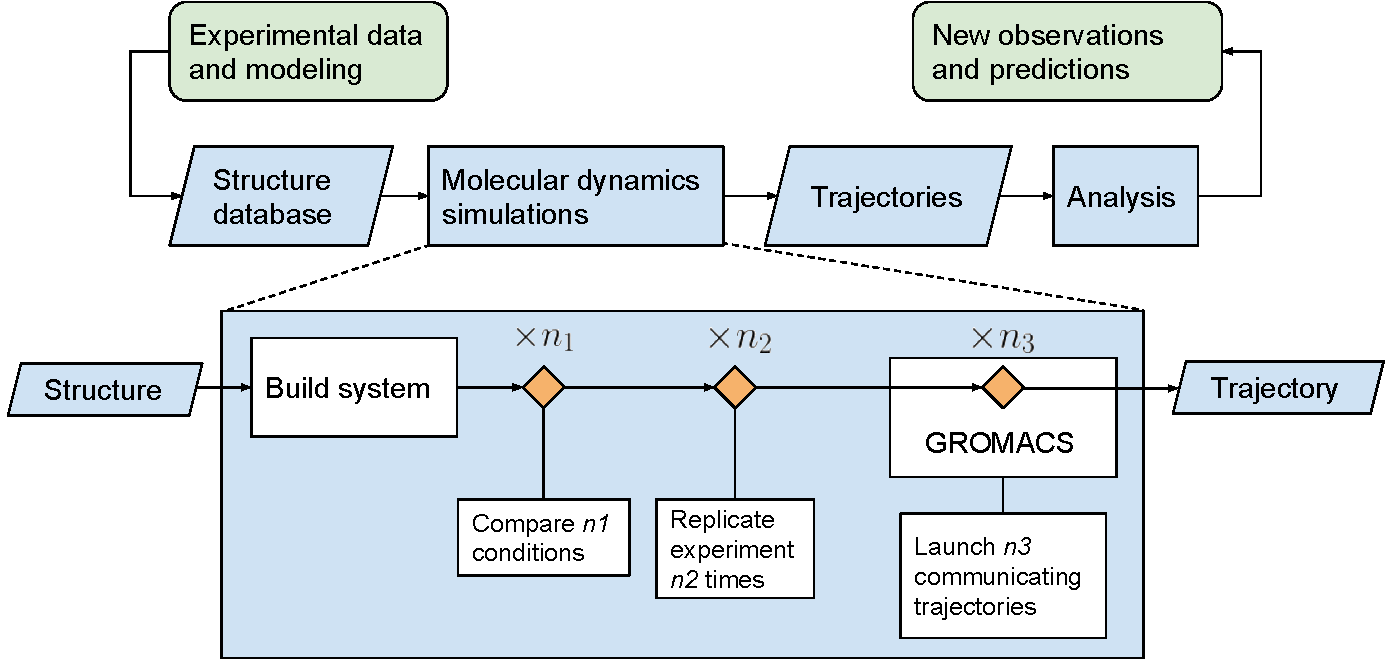
\includegraphics[width=1\textwidth]{figs/md-workflow.pdf}
\caption{\label{fig:mdworkflow}
\textbf{An MD workflow.} 
MD Simulations take experimental data and modeling (green, top-left) of complex, biomolecular sytems as input to generate trajectories that can subsequently be analyzed to extract biological insight and predictions (green, top-right). Carrying out the MD simulations can be complex in a realistc scientific application (bottom) since multiple ensembles of trajectories need to be generated (bottom). 
}
\end{figure*}

A critical question, that we approach here, is how to distribute compute resources efficiently in the simulation design. 
When increasing the machines size, one can choose to either add more independent trajectories (increase $n_2$), more communicating trajectories (increase $n_3$) or make simulations longer by increasing the number of compute nodes per MD trajectory,  $N$. Currently generally these parameters are chosen \textit{ad hoc}, or by iterating  post-simulation analysis.
The optimal choice of these parameters, depends on the scaling properties along these different parameter axes. The use cases presented in this report thus aim to  elucidate these properties.
Furthermore, some of these parameter choices have potential to be automated, in FE calculations e.g. by extending or adding trajectories until a given error measure is below a given tolerance. This would greatly improve usability and the efficiency of MD simulations. 

\section{Aims}
The main aim is to implement one or more realistic large-scale use case to benchmark scalability of GROMACS for FE calculations. The use cases will also be used as tutorial material and as templates for the novice user. 

%\section{Results}
\section{Use case I: DNA base pair opening}

\subsection{Biological relevance and scientific aims}
The DNA molecule encodes biological information that has to be protected from chemical exposure while being accessible to read, modify and repair. It typically exists in a double-helical form in which two complementary strands intertwine and bind through Watson-Crick (WC) hydrogen-bonding between the bases, providing a stabilizing environment for the base pairs. However, the base pairs can open up, spontaneously or in the presence of an enzyme, allowing for a base to flip out from the helix~\cite{knips2017both}. The closed, base-paired and the open, base-flipped state are illustrated in Fig.~\ref{fig:dnastates}. The propensity for base pair opening  is sequence dependent, but it is not know exactly how and there is only limited amount of experimental data available and only for certain  base pairs and sequences. There is als growing interest in studying base pair opening to elucidate the equilibrium between canonical WC basepair and the less well-known Hoogsteen basepair, and how it links to DNA sequnce, structure and function~\cite{chakraborty2017energy}.
\begin{figure*}[thbp!]
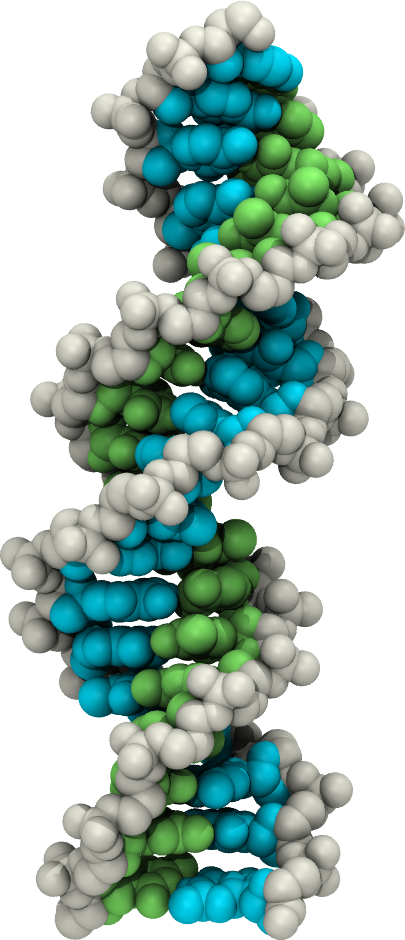
\includegraphics[height=8cm]{figs/dna-helix-closed.png}
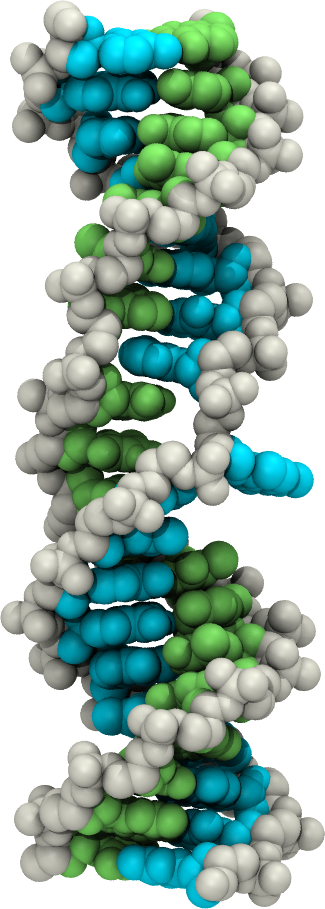
\includegraphics[height=8cm]{figs/dna-helix-flip.png}
\caption{\label{fig:dnastates}
\textbf{DNA structure and base pair opening} Base pairs in the DNA double-helical structure can spontaneously open up, which is necessary for exposing the bases to the chemical environment, or for the DNA strands to ``unzip''.
}
\end{figure*}

\subsection{The need for large-scale simulations}
The mechanisms for base pair opening and the importance of the local and global DNA sequence have been investigated for MD simulation~\cite{lindahl2017sequence}. However, because of the combinatorics of systematically scanning multiple sequences and target basepairs in FE calulcations it is only recently that advances in sampling methods and computational power have allowd for MD simulations to properly address  these questions.
With MD simulations the free energy of opening, acting as a direct measure of the propensity for opening,
 can be calculated for any base pair in any DNA sequence. Calculating the free energy for all the base pairs in a sequence and for a large database of sequences of interest, makes this an inherently large-scale and parallelizable problem. 

\subsection{Methods and system setup}
The system is set up the same as in Ref.~\cite{lindahl2017sequence}. The main ingredients are summarized here.
We use the Accelerated Weight Histogram (AWH)~\cite{lindahl2014accelerated}, available in GROMACS~2018, to calculate the potential of mean force (PMF) along a reaction coordinate (RC) characterizing the opening. The RC is definesd as a simple distance between the two bases in a target base pair. % Multiple communicating AWH walkers can be launched simultaneously (using the \texttt{gmx mdrun  -multi} command.
Here we use a  3-turn DNA helix, 20 basepairs long. The DNA strands are periodically connected, emulating an infinitely long helix. This helps by allowing for having a small box size. In this case the 9365-atom system consists of about 87\% solvent. For a more ``generous'' build, using a dodecahedron box and non-periodic DNA, a 19-mer long DNA chain requires 45666 atoms, where about 97\% is solvent Ref.~\cite{lindahl2017sequence}, i.e.\ both bigger and higher concentration of water and ions.

\subsection{General applicability}
\cite{zhang2018accurate}

\subsection{Strong scaling, the number of nodes per trajectory ($N$)}
Because of the small system size, the represents a challenging test case. It is however representative for many realistic use-cases. %, e.g. in drug-design. 
\begin{figure*}[thbp!]
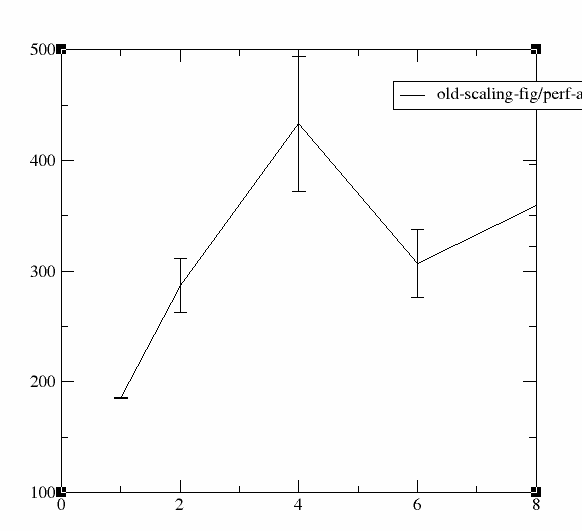
\includegraphics[height=5cm]{figs/dna-strong-scaling-screenshot.png}
\caption{\label{fig:dnastrongscaling}
\textbf{Strong scaling for the DNA system} TODO. 
}
\end{figure*}

\subsection{Walker scaling: the number of communicating trajectories ($n_3$)}

%\subsection{Independent walker scaling: the number of independent trajectories ($n_2$)}



\section{Use case II: permeability and selectivity of aquaporin membrane channel}
\subsection{Biological relevance and scientific aims}
\cite{lindahl2018permeability}
\subsection{Methods and system setup}

\section{Summary/Outlook}

\bibliography{summary}


\end{document}
